\clearpage

\section{Results for $\sin^2\theta_{23}$ and vacuum oscillation probabilities}
\label{appendix:vacuum_results}

%
% ----------------------------------------
%

%best fit value
`2+N' 3-flavour $\nu_{\mu}$-disappearance fits were performed on the combined 3.010$\times$10$^{20}$ 
POT Run 1+2+3 dataset using the method described in section \ref{sec:oscfit}, $\sin^2\theta_{23}$ instead of 
$\sin^22\theta_{23}$, and 3-flavour oscillation probabilities in vacuum instead of matter.
This analysis found
$|\Delta m^{2}_{32}|$ = 2.442$\times$10$^{-3}$ $eV^{2}/c^{4}$ and
$\sin^{2}\theta_{23}$ = 0.513
to be the best-fit values.
At the best-fit point, N$_{exp}$ is 57.90
and $\chi^2_{bf}$/$ndf$ = 56.03/71.

%pulls
The pulls, defined in Eq.\ \ref{eqn:bfpull}, of all 48 systematic parameters allowed to float in the fit are shown in
Fig.\ \ref{fig:results_data123_pulls_vacuum}.
From this figure, it is apparent that most systematic parameters barely move from their nominal values.

\begin{figure*}[htb]
\center
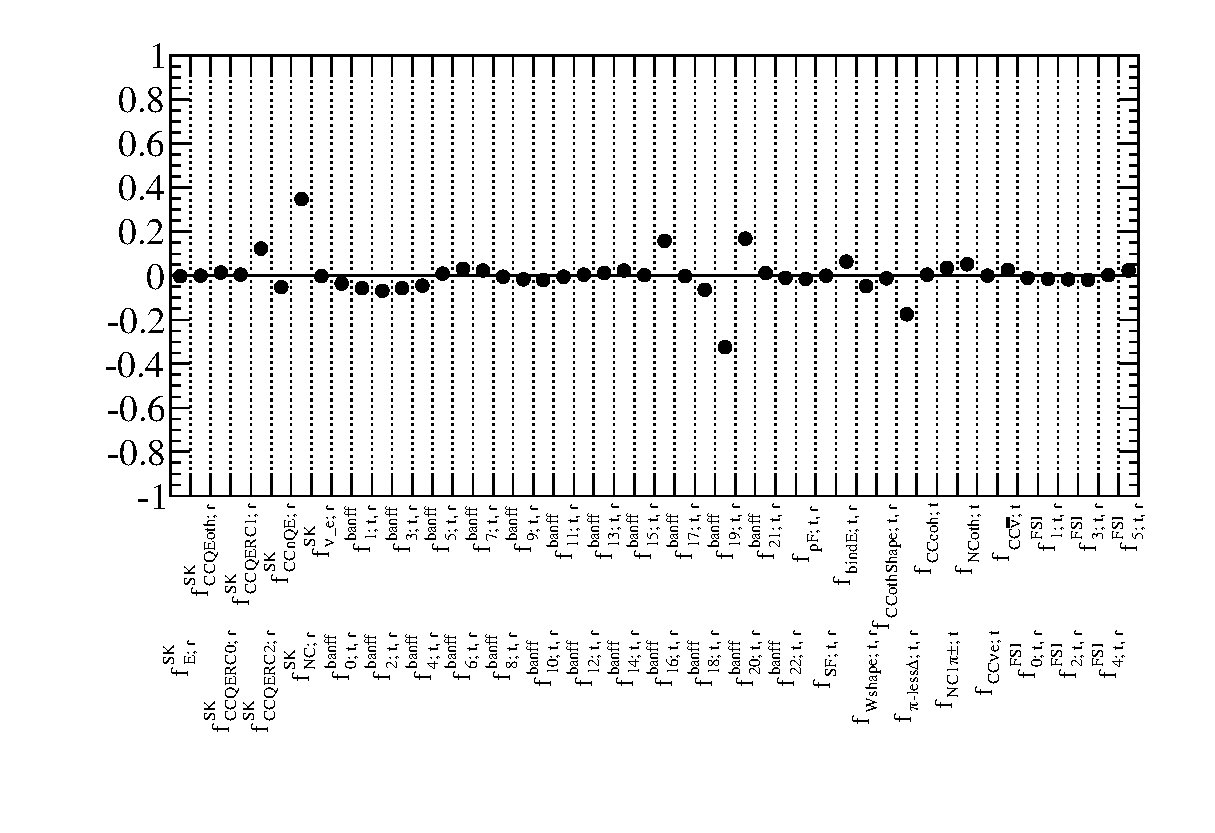
\includegraphics[width=50pc,angle=270]{./images/fit_data/vacuum/pulls_3}
\caption {
  Systematic parameter pulls for the `2+N' $\sin^2\theta_{23}$ in vacuum fit to the Run 1+2+3 dataset.
}
\label{fig:results_data123_pulls_vacuum}
\end{figure*}

%goodness of fit
% A goodness-of-fit test was performed as described in Sec.\ \ref{sec:gof_test}.
% The $\chi^2$ distributions from 
% which the p-values were calculated are shown in Fig.\ \ref{fig:results_data123_goodness_vacuum}.
% {\color{red}The fit has a high degree of plausibility.}

% \begin{figure*}[htb]
% \center
% \includegraphics[width=18pc]{./images/fit_data/vacuum/goodness_3}
% \caption {
%   Distribution of $\chi^2_{gof}$, the goodness-of-fit (gof) $\chi^2$, 
%   from 1k toy MC experiments generated at the `2+N' $\sin^2\theta_{23}$ in vacuum Run 1+2+3 best-fit oscillation point.
%   The $\chi^2_{gof}$ value for the Run 1+2+3 data ($\chi^2_{data}$) is highlighted.
% }
% \label{fig:results_data123_goodness_vacuum}
% \end{figure*}


%spectra
The reconstructed neutrino energy distribution of the single $\mu$-like ring events in the Run 1+2+3 dataset is shown in Fig.\ 
\ref{fig:results_data123_spectrum_vacuum} along with the `2+N' $\sin^2\theta_{23}$ in vacuum best-fit prediction and
the prediction made under the no-oscillation 
hypothesis. Also shown is the ratio between the data and the no-oscillation spectrum and the ratio between the `2+N' $\sin^2\theta_{23}$ in vacuum best-fit 
spectrum and the the no-oscillation spectrum; in both of these ratios, the characteristic energy-dependent deficit can be 
clearly seen.
These distributions are shown in the 73-bin scheme in reconstructed 
neutrino energy that was used in the fitting procedure (see Sec.\ \ref{sec:mc_templates:template_binning}).
Fig.\ \ref{fig:results_data123_spectrum_coarse_vacuum} shows the same distributions in the coarse binning scheme
(see Sec.\ \ref{sec:results_bestfit_spectra}).

\begin{figure*}[htb]
\center
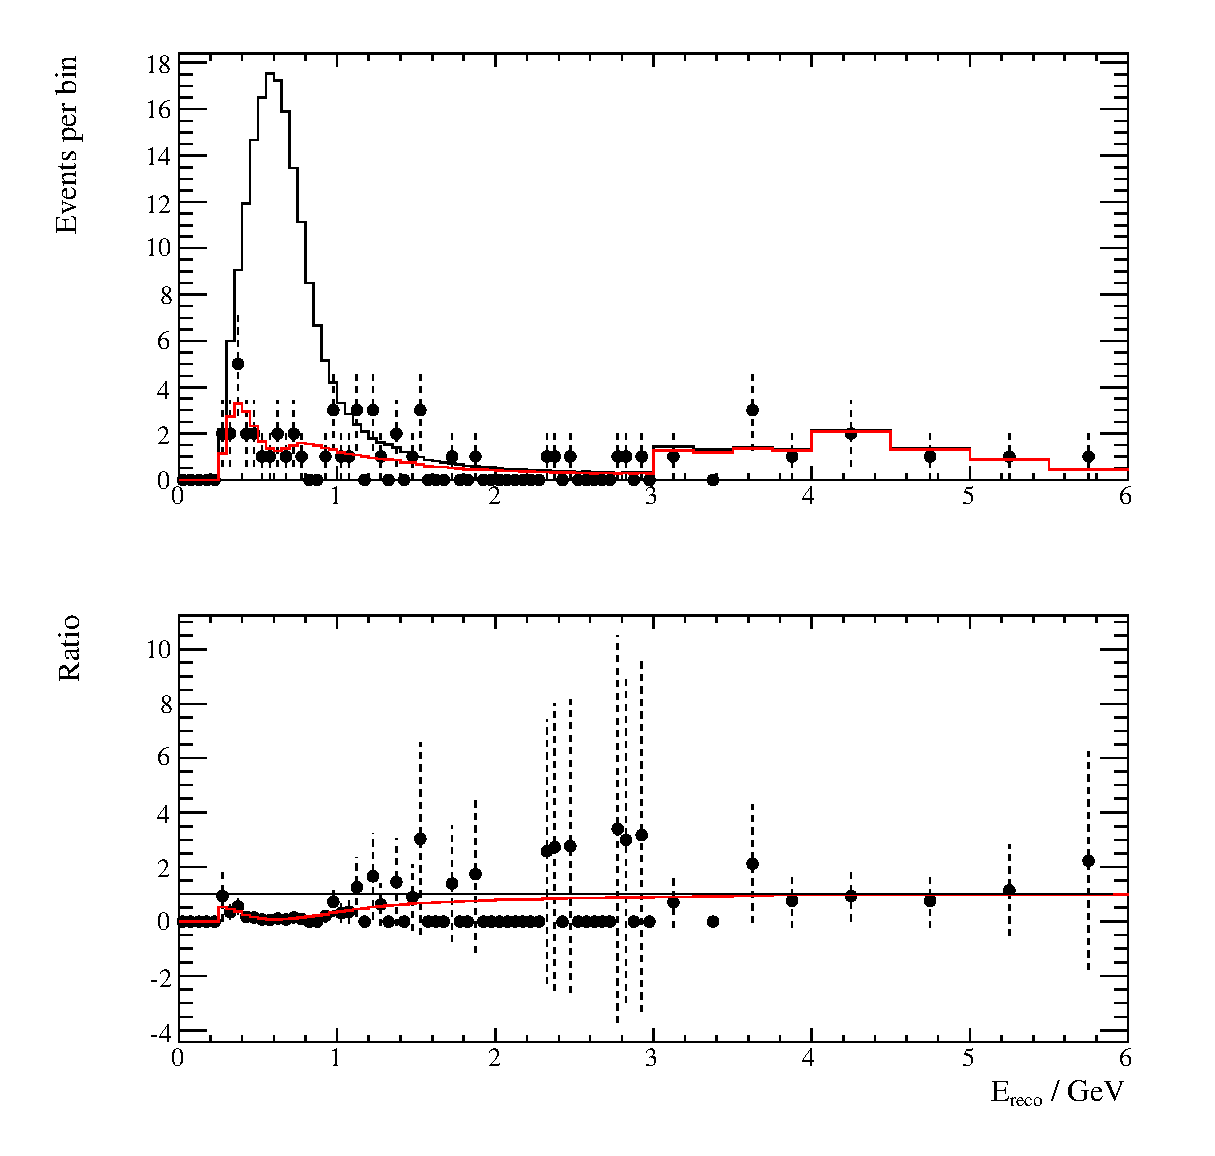
\includegraphics[width=28pc]{./images/fit_data/vacuum/spectrum_3}
\caption {
  Best-fit reconstructed energy spectrum (top) obtained from the `2+N' $\sin^2\theta_{23}$ in vacuum fit to the combined Run 1+2+3 dataset.
  The Run 1+2+3 dataset and the prediction obtained from the no-oscillation hypothesis are also shown.
  The spectra are shown using the 73 bins used in the fit (see Sec.\ \ref{sec:mc_templates:template_binning}).
  The ratio of the data and best-fit distribution to the no-oscillation hypothesis is shown 
  in the bottom plot. The characteristic energy-dependent deficit can be clearly seen.
}
\label{fig:results_data123_spectrum_vacuum}
\end{figure*}


\begin{figure*}[htb]
\center
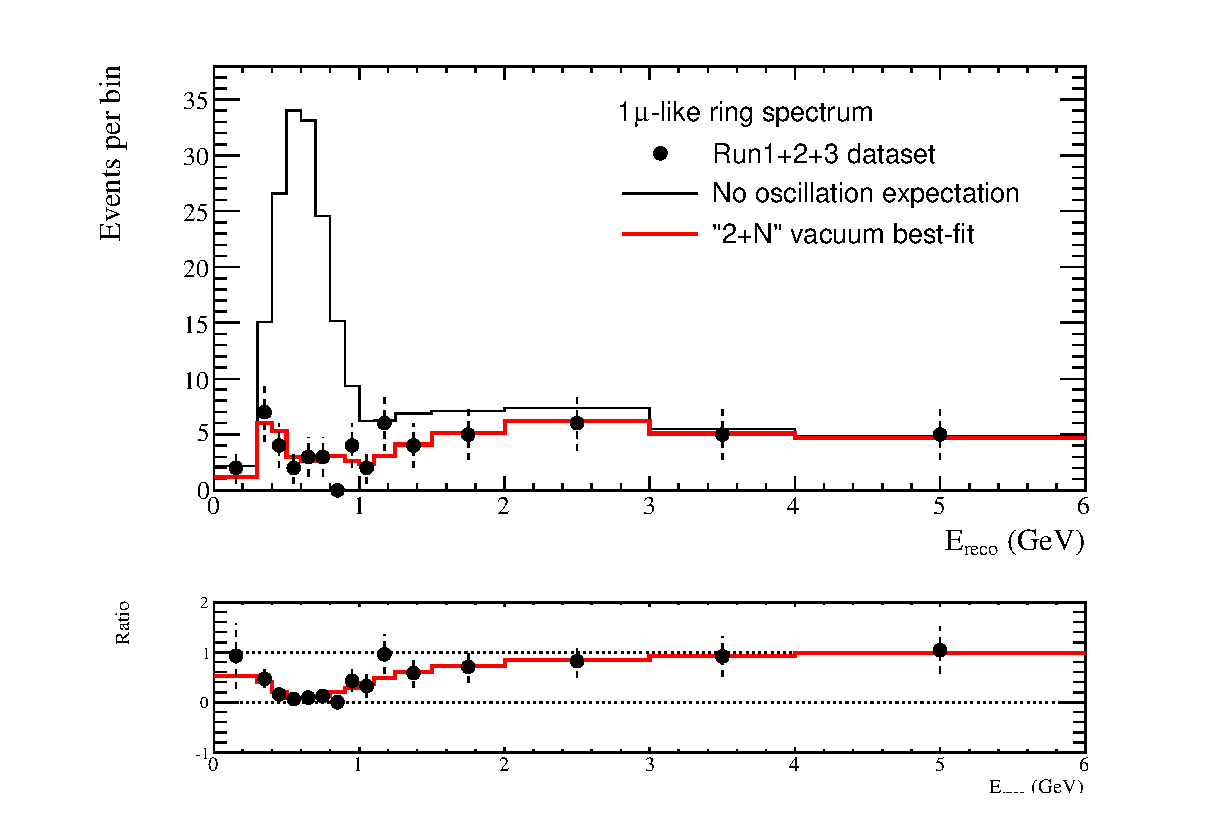
\includegraphics[width=34pc]{./images/fit_data/vacuum/spectrum_and_ratio_coarse.eps}
\caption {
  Best-fit reconstructed energy spectrum using the coarse binning scheme (see 
  Sec.\ \ref{sec:results_bestfit_spectra}) obtained from the `2+N' $\sin^2\theta_{23}$ in vacuum fit to the Run 1+2+3 dataset.
  Also shown are the spectrum obtained under the no-oscillation hypothesis
  and the ratios of the data and best-fit spectrum to it.
}
\label{fig:results_data123_spectrum_coarse_vacuum}
\end{figure*}


%dchisq surface
The $\Delta\chi^2$ surface for the the `2+N' $\sin^2\theta_{23}$ in vacuum fit to the Run 1+2+3 dataset is shown in Fig.\
\ref{fig:results_data123_chisq_vacuum}, 
as a function of $\sin^{2}\theta_{23}$ and $|\Delta m^{2}_{32}|$.

The 68\% and 90\% CL regions for the `2+N' $\sin^2\theta_{23}$ in vacuum fit to the Run 1+2+3 dataset are shown using the constant-
$\Delta\chi^2$ method in Fig.\ \ref{fig:results_data123_contour_vacuum}.

A comparison between the $\sin^2\theta_{23}$ contours assuming vacuum and matter using the constant-$\Delta\chi^2$ method
is shown in Fig.\ \ref{fig:results_compare_contours_matter_vacuum}.

\begin{figure*}[htb]
\center
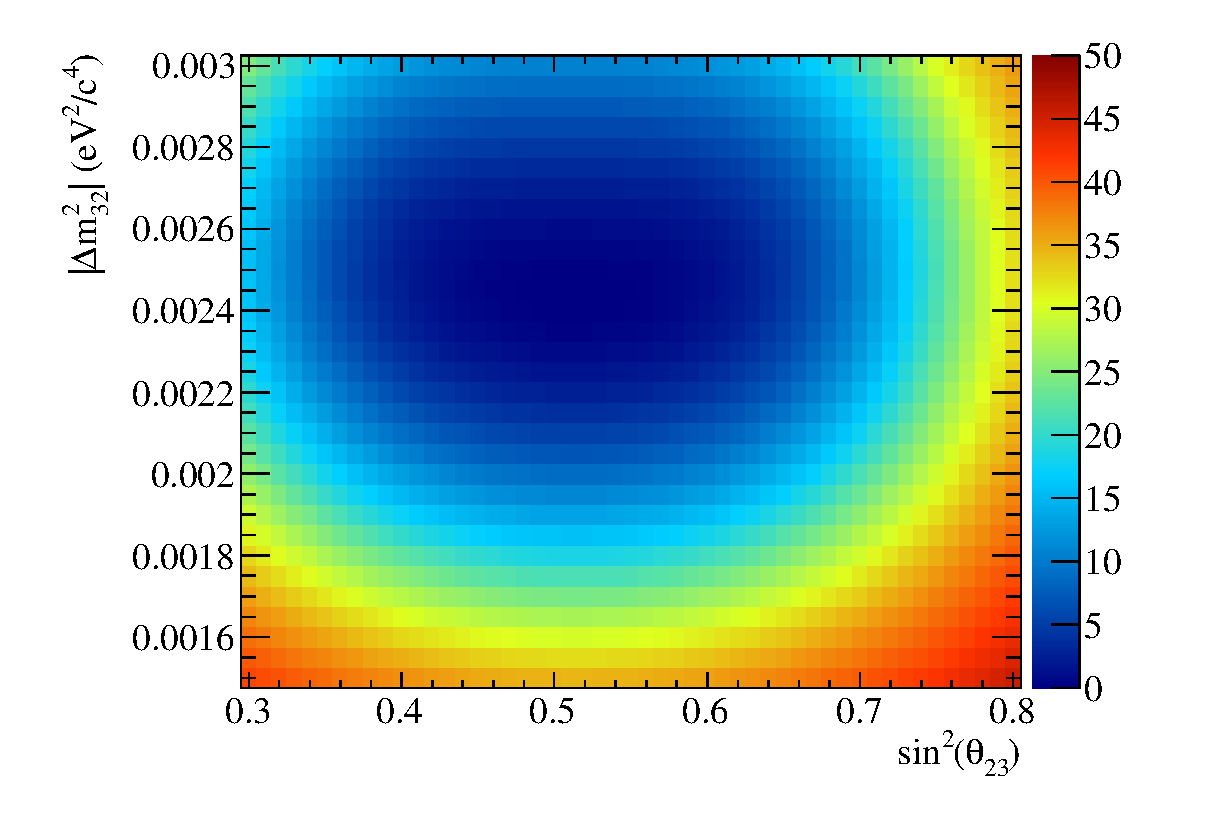
\includegraphics[width=30pc]{./images/fit_data/vacuum/dchisq_3}
\caption {
  $\Delta\chi^2$ surface for the `2+N' $\sin^2\theta_{23}$ in vacuum fit to the Run 1+2+3 dataset.
}
\label{fig:results_data123_chisq_vacuum}
\end{figure*}


\begin{figure*}[htb]
\center
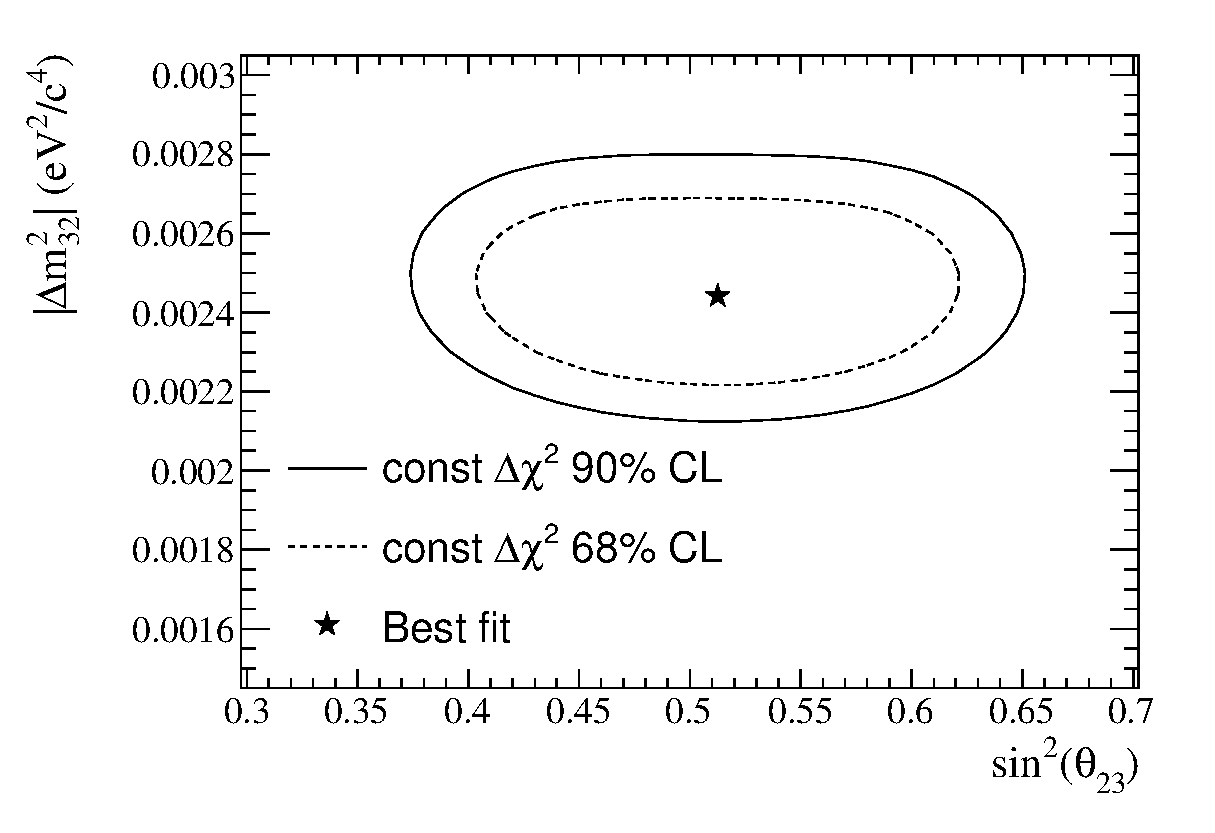
\includegraphics[width=30pc]{./images/fit_data/vacuum/contours_3}
\caption {
  68\% CL and 90\% CL allowed region (including systematics), 
  constructed with the constant-$\Delta\chi^{2}$ method,
  for the `2+N' $\sin^2\theta_{23}$ in vacuum fit to the Run 1+2+3 dataset.
  The `2+N' best-fit point is also shown.
}
\label{fig:results_data123_contour_vacuum}
\end{figure*}


\begin{figure*}[htb]
\center
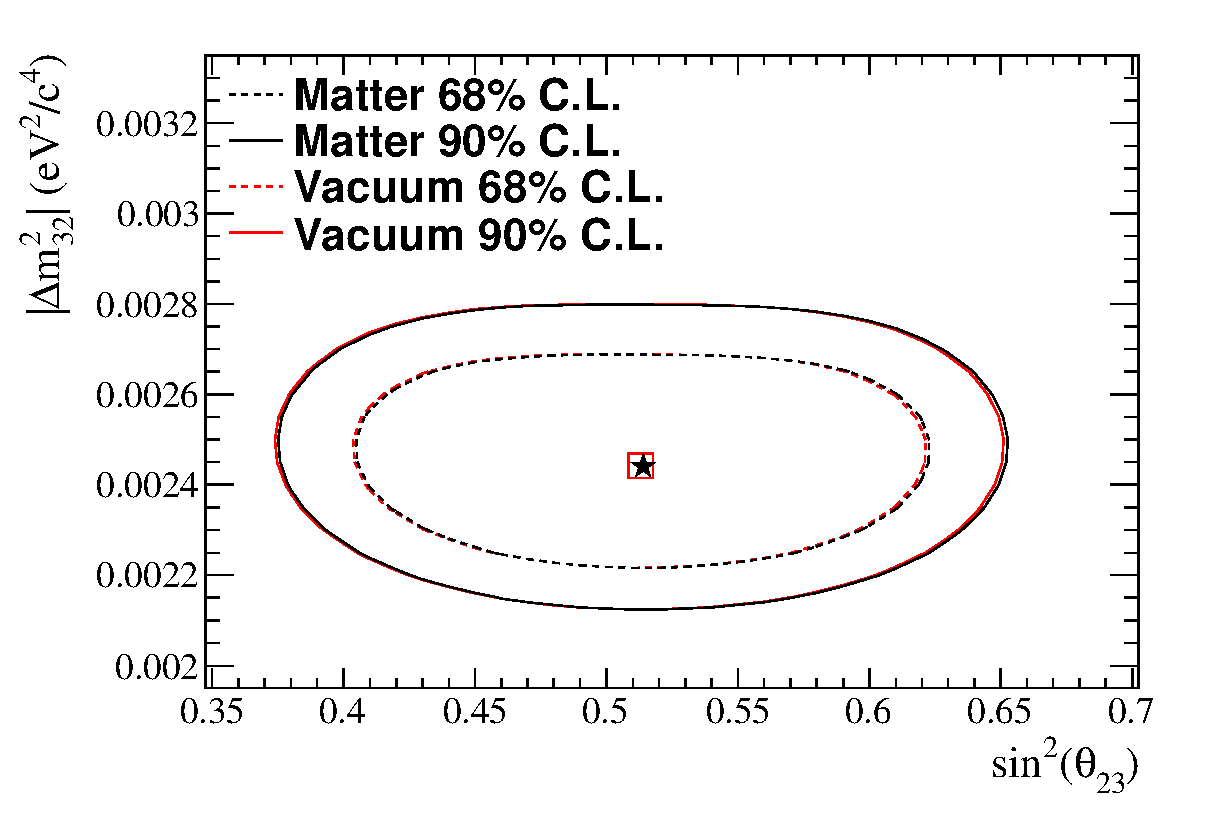
\includegraphics[width=35pc]{./images/fit_data/compare/contour_compare_octants_vacuum}
\caption {
  Comparison between the `2+N'
  68\% CL and 90\% CL allowed regions
  for the $\sin^2\theta_{23}$ in vacuum and $\sin^2\theta_{23}$ in matter fits
  obtained using the constant-$\Delta\chi^2$ method. 
  The comparison is shown for the fits to the Run 1+2+3 dataset.
}
\label{fig:results_compare_contours_matter_vacuum}
\end{figure*}
